\section{Foresight in the engine}\label{app:foresight}
Four jobs ran oracle policies in the engine, each on a rented RTX 5090 machine with weaker host memory than host B's. Jobs 093--097 report ratios of mean speeds rather than of mean times per token; recomputed either way, no ratio
moves by more than \fxMeanKindDiffMax.
The fourth (096) is the confirmatory factorial of \cref{fig:factorial}: ten configurations per cell, each in a fresh
context, in an order shuffled per cell with a recorded seed, on hosts O4 (Ryzen 9 9950X: \fxCpuFour, \fxLinkFour{} and
\fxBestFour\,GB/s by the CPU, over the link and at best) and O5 (Ryzen 9 9950X3D: \fxCpuFive, \fxLinkFive{} and
\fxBestFive\,GB/s), with ten predictions per machine committed before either started
(\texttt{prereg/foresight\_outcome\_096.md}). They held at most cells. The failures: \MinOne's gain above the predicted band at Qwen3 25\% on O4 and different
between the two machines by up to \fxFetchSpreadMax{} against the 0.15 predicted; \cfg{Belady-1R} faster than
predicted at Qwen3 12.5\% on O4, with reads below the predicted 1.25--1.9$\times$ those of the \emph{ahead-only} oracle (below) at Qwen3 12.5\% on
both machines and at gpt-oss 11\% on O4 (down to \fxNbReadsOverLeadMin$\times$); the bytes share at Qwen3 12.5\% on O4
(\amBytesHostMax\% of the gap against a predicted 25--55\%); and the reads \DepOne{} saves at gpt-oss 40\% on O5,
just above the predicted 22\%. \DepOne{} came to \fxFoaHostMin--\fxFoaHostMax$\times$ the deployed cache at the host-bound cells, at the bottom of the predicted 0.97--1.12$\times$ although its reads fell as predicted, and to \fxFoaGpuFiveMin--\fxFoaGpuFourMax$\times$ at the GPU-bound cells.
\Cref{tab:single_read} lists every cell of the single-read factorial of \cref{sec:foresight} on host O3 (a Ryzen 9 9950X
whose probe reads \fsfHostCpu\,GB/s by the CPU at the helper count, \fsfHostLink{} over the link, \fsfHostBoth{} with
both and \fsfHostMax{} at best; the model's FETCH tables \texttt{0,0,1,2,2} for gpt-oss and \texttt{0,0,1,1,2,3,4,4,5}
for Qwen3), and \cref{tab:accounting_measured} the milliseconds per token of the engine states the three jobs
realised beside each machine's bound and the model's values. \Cref{tab:foresight} lists the first job (093),
\cfg{Belady-2R} with a window sweep on host O1 (a Ryzen 9 9950X: \fsmHostCpu, \fsmHostLink, \fsmHostBoth{} and
\fsmHostMax\,GB/s; tables \texttt{0,0,1,2,3} and \texttt{0,0,1,2,3,4,5,6,7}), and \cref{tab:foresight_bytes} the
second (094), \MinTwo{} beside \cfg{Belady-2R} on host O2 (a Ryzen 9 7950X:
\fsbHostCpu, \fsbHostLink, \fsbHostBoth{} and \fsbHostMax\,GB/s; the same tables). On O1 and O2 every cell but
gpt-oss 40\% and Qwen3 43.75\% is host-bound in \cref{eq:limit}; on O3, whose memory is stronger, the same four.

\paragraph{The single-read oracles.} In \MinOne{} the step's plan is computed before the layer runs from the
trace's record of the current step: the misses MIN with bypass would admit are fetched by the engine's FETCH
operation into their victims' slots and run from there, and every other miss runs on the CPU; the oracle refuses an
admission when no resident's next use is further than the candidate's. Reading ahead admits, each step,
the non-resident experts whose first use is at least $d$ steps away ($d{=}2$ unpaced, 3 paced), provided the victim's
next use is further than the candidate's use after that first one; an expert used sooner than $d$ steps away misses
on the CPU (the \emph{ahead-only} oracle), or is fetched as in \MinOne{} (the read-ahead oracle; paced with $d{=}3$, the form of
\cref{tab:configs}). The same policies simulated on the trace with the engine's
semantics (the lookahead within the sequence, residents carried over with their next use recomputed at each sequence
start) predict the engine's reads and hit rates: \MinOne's hit rate within \fsfSimHitDiffMax{} points and its
reads within \fsfSimReadsDiffMin{} to \fsfSimReadsDiffMax\%, the read-ahead oracle's hits within two points
(\cref{tab:single_read}). Simulated, \MinOne{} reads $R^\star_{\mathrm{eng}}$ experts per token, MIN's count in the
engine: its window ends at the problem's end, and an expert served in a step stays for that step. The simulator the job's predictions were registered against gave a resident carried over
from the previous sequence no next use, so it was evicted first; that over-counted \MinOne's reads by 17\%
at the two GPU-bound cells, which is why two of its reads clauses failed (\cref{app:prereg}). Each configuration of
\texttt{llama-ec-bench} starts with a cold cache in a fresh context. The paced copy path copies one 16\,MB piece at a time on a single copier thread and
publishes a landed copy at the start of the next step; the unpaced path copies each admission as one transfer. The
background admissions of \cfg{Belady-2R} drive host memory at \fshHostUtilMin--\fshHostUtilMax\% of the probe's best
rate at the host-bound cells, the single-read oracles that read ahead at \fsPrefetchHostUtilMin--\fsPrefetchHostUtilMax\%
(the paced read-ahead oracle \fsbpHostUtilMin--\fsbpHostUtilMax\%), the deployed cache itself at \fsBaseHostUtilMin--\fsBaseHostUtilMax\%,
\MinOne{} at \fsfHostUtilMin--\fsfHostUtilMax\%. The predictions and their outcomes are in
\texttt{prereg/foresight\_outcome\_095.md}: of 56 clauses, 44 held and 12 failed, all of size (\cref{app:prereg}).

% generated by scripts/foresight_paper.py from prereg/foresight_095.json and prereg/foresight_single_read_sim.json
\begin{table*}[t]\centering\scriptsize\setlength{\tabcolsep}{2.2pt}
\caption{The single-read oracles (job 095; RTX 5090, Ryzen 9 9950X, host memory \fsfHostMax\,GB/s at best) beside \cfg{Belady-2R}. Per cell: the deployed cache's speed and its share of this machine's bound; for each oracle with the whole sequence in view, its ratio to the deployed cache (paired, 95\% interval), hit rate, host reads per token (CPU misses + fetches + admissions) as a multiple of $R^\star$ (each read counted once), share of the bound and the calibrated model on its own counters against its measured time. \MinOne: MIN with bypass, admitted misses fetched into their slot this step; \emph{ahead only}: MIN's admissions copied when their first use is at least two steps away, other misses served by the CPU; \emph{read-ahead}: \MinOne{} and ahead only together; \emph{read-ahead, paced}: the same on the paced copy path with a three-step lead (the read-ahead oracle of \cref{tab:configs}); \cfg{Belady-2R}: Belady's rule without bypass, unpaced. The simulation columns give the trace's prediction of reads and hits for \MinOne{} (its reads are $R^\star_{\mathrm{eng}}$, \cref{app:foresight}) and the read-ahead oracle.}
\label{tab:single_read}
\resizebox{\textwidth}{!}{%
\begin{tabular}{@{}lrr|lrrrr|lrrr|lrrr|lr|lr|rrrr@{}}\toprule
 & \multicolumn{2}{c|}{deployed} & \multicolumn{5}{c|}{\MinOne} & \multicolumn{4}{c|}{read-ahead} & \multicolumn{4}{c|}{\cfg{Belady-2R}} & \multicolumn{2}{c|}{ahead only} & \multicolumn{2}{c|}{read-ahead, paced} & \multicolumn{2}{c}{sim.\ \MinOne} & \multicolumn{2}{c}{sim.\ read-ahead} \\
Cell & tok/s & \% bound & ratio & hits & reads$/R^\star$ & \% bound & model & ratio & hits & reads$/R^\star$ & \% bound & ratio & hits & reads$/R^\star$ & \% bound & ratio & \% bound & ratio & \% bound & $R^\star_{\mathrm{eng}}$ & hits & reads & hits \\\midrule
gpt-oss 11\% & 55.5 & 46 & 1.29 [1.28, 1.29] & 72 & 1.04 & 59 & -8\% & 1.39 [1.39, 1.40] & 86 & 1.23 & 64 & 0.91 [0.90, 0.92] & 98 & 1.77 & 42 & 1.26 & 58 & 1.45 & 67 & 39 & 73 & 46 & 87 \\
gpt-oss 25\% & 90.3 & 30 & 1.32 [1.31, 1.33] & 89 & 1.08 & 39 & -13\% & 1.49 [1.48, 1.50] & 97 & 1.45 & 44 & 1.14 [1.12, 1.15] & 99 & 2.11 & 34 & 1.45 & 43 & 1.66 & 50 & 16 & 89 & 22 & 99 \\
gpt-oss 40\% & 128.8 & 25 & 1.25 [1.24, 1.27] & 95 & 1.14 & 32 & -14\% & 1.39 [1.37, 1.41] & 99 & 1.60 & 35 & 1.27 [1.25, 1.28] & 99 & 2.20 & 32 & 1.38 & 35 & 1.49 & 38 & 7 & 95 & 12 & 100 \\
Qwen3 12.5\% & 32.3 & 48 & 1.34 [1.34, 1.35] & 74 & 1.04 & 64 & -9\% & 1.42 [1.41, 1.43] & 84 & 1.20 & 68 & 0.69 [0.68, 0.71] & 77 & 2.47 & 33 & 1.22 & 58 & 1.41 & 68 & 100 & 74 & 115 & 84 \\
Qwen3 25\% & 51.8 & 34 & 1.38 [1.37, 1.39] & 88 & 1.04 & 48 & -15\% & 1.48 [1.46, 1.49] & 96 & 1.42 & 51 & 1.06 [1.05, 1.08] & 99 & 2.00 & 37 & 1.41 & 48 & 1.67 & 57 & 45 & 88 & 61 & 97 \\
Qwen3 43.75\% & 91.4 & 30 & 1.26 [1.25, 1.28] & 96 & 1.08 & 38 & -17\% & 1.41 [1.39, 1.42] & 99 & 1.62 & 42 & 1.27 [1.26, 1.29] & 100 & 2.29 & 38 & 1.40 & 42 & 1.50 & 45 & 15 & 96 & 23 & 100 \\
\bottomrule\end{tabular}}\end{table*}

% generated by scripts/accounting_measured.py
\begin{table*}[t]\centering\scriptsize\setlength{\tabcolsep}{3pt}
\caption{The accounting, measured: milliseconds per token of the engine's states that the oracle jobs realised, on each oracle host, beside that host's limit and the model's values for the states it prices. \emph{online}: the deployed policy; \emph{no ovl.}: its within-layer overlap off; \emph{all CPU}: no FETCH table; \emph{bypass}: MIN with bypass with background admissions (two reads per admitted expert); \emph{hit-opt.}: Belady prefetch (two reads); \emph{fetch}: MIN with bypass, admitted misses fetched into their slot (one read, serialised: the model's foresight-only state $v(F)$); \emph{both}: fetch and the scheduled single-read prefetch (one read, overlapped: the model's $v(O,F)$); \emph{limit}: the limit on that host; $v(F)$, $v(O,F)$, $v(\mathrm{all})$: the model.}
\label{tab:accounting_measured}
\begin{tabular}{@{}llr|rrrr|rr|r|rrr@{}}\toprule
Host & Cell & online & no ovl. & all CPU & bypass & hit-opt. & fetch & both & limit & $v(F)$ & $v(O,F)$ & $v(\mathrm{all})$ \\\midrule
Ryzen 9 9950X (093) & gpt-oss 11% & 21.12 & 21.01 & 22.91 & -- & 22.88 & -- & -- & 10.06 & 14.54 & 11.27 & 10.06 \\
Ryzen 9 9950X (093) & gpt-oss 25% & 12.89 & 12.91 & 14.21 & -- & 9.22 & -- & -- & 4.03 & 8.04 & 5.10 & 4.03 \\
Ryzen 9 9950X (093) & gpt-oss 40% & 8.90 & 8.95 & -- & -- & 5.99 & -- & -- & 1.97 & 5.75 & 3.84 & 1.97 \\
Ryzen 9 9950X (093) & Qwen3 12.5% & 36.92 & 36.91 & 43.29 & -- & 40.29 & -- & -- & 18.04 & 24.90 & 19.29 & 18.04 \\
Ryzen 9 9950X (093) & Qwen3 25% & 22.73 & 22.76 & 26.60 & -- & 18.22 & -- & -- & 8.11 & 14.04 & 9.22 & 8.11 \\
Ryzen 9 9950X (093) & Qwen3 43.75% & 12.71 & 12.67 & -- & -- & 8.12 & -- & -- & 3.32 & 8.25 & 5.51 & 3.32 \\
Ryzen 9 7950X (094) & gpt-oss 11% & 20.85 & -- & -- & 20.17 & 21.57 & -- & -- & 10.04 & 14.27 & 11.96 & 10.04 \\
Ryzen 9 7950X (094) & gpt-oss 25% & 12.72 & -- & -- & 10.77 & 7.80 & -- & -- & 4.02 & 7.86 & 5.86 & 4.02 \\
Ryzen 9 7950X (094) & gpt-oss 40% & 8.79 & -- & -- & 7.13 & 5.62 & -- & -- & 1.97 & 5.63 & 3.78 & 1.97 \\
Ryzen 9 7950X (094) & Qwen3 12.5% & 36.64 & -- & -- & 36.58 & 38.74 & -- & -- & 18.00 & 24.70 & 20.06 & 18.00 \\
Ryzen 9 7950X (094) & Qwen3 25% & 22.24 & -- & -- & 19.67 & 15.80 & -- & -- & 8.09 & 13.58 & 9.90 & 8.09 \\
Ryzen 9 7950X (094) & Qwen3 43.75% & 12.02 & -- & -- & 10.11 & 7.42 & -- & -- & 3.32 & 7.56 & 4.90 & 3.32 \\
\bottomrule\end{tabular}\end{table*}


\begin{figure}[t]\centering
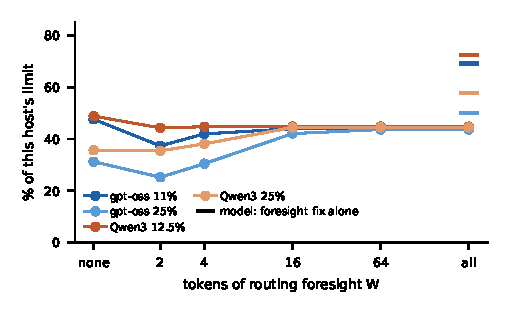
\includegraphics[width=0.5\linewidth]{figs/foresight.pdf}
\caption{The first oracle job (093, host O1): speed as a percentage of this machine's bound against the window $W$ of
future routing \cfg{Belady-2R} sees, at the four host-bound cells. ``none'' is the deployed cache; ``all'' the
whole sequence; points are connected for the trend only. The tick at the right is the model's foresight-only term for
the cell, the speed it predicts with that one fix; the oracle's host traffic sits at \fsmUtilWinMin--\fsmUtilWinMax\%
of the probe's best rate at every window, so its speed is $R^\star$ over its reads times that utilisation,
\fsmHostFracMin--\fsmHostFracMax\% of the bound with the whole sequence in view.}
\label{fig:foresight}
\end{figure}

\paragraph{The double-reading oracles.} \cfg{Belady-2R} and \MinTwo{} read the routing of the next $W$ decode steps; their copies ride the
paced admission path, and an expert still in flight at its step runs on the CPU like any other miss. \cfg{Belady-2R},
the \emph{hit-optimal} oracle, admits the experts those steps will route to, soonest first, evicting the resident whose
next use is furthest (Belady within the window), for one future use as readily as for ten. \MinTwo, the \emph{bytes-optimal}
oracle, is MIN with bypass with its admissions made through the background path: a miss is served where it is, by the
CPU or a demand copy, and admitted only if its next use comes before the furthest next use among the residents. With
the whole sequence in view \cfg{Belady-2R} runs \fsmRatioGMid$\times$ [\fsmRatioLoGMid, \fsmRatioHiGMid] the
deployed cache at gpt-oss 25\% and \fsmRatioQMid$\times$ [\fsmRatioLoQMid, \fsmRatioHiQMid] at Qwen3 25\% on host O1,
\fspRatioGMid$\times$ and \fspRatioQMid$\times$ on O2, and \fsHitGpuMin--\fsHitGpuMax$\times$ at the two GPU-bound
cells; half of its gain at gpt-oss 25\% arrives between $W{=}4$ and 16 (\fsmWfiftyGMid{} tokens by log
interpolation; Qwen3 25\%: \fsmWfiftyQMid{} against the trace's 3.9). Where the host binds hardest it loses,
\fsHitLossMin--\fsHitLossMax\% at gpt-oss 11\% and Qwen3 12.5\% on both machines, and at every window on O1
(\fsmNegWinMin--\fsmNegWinMax$\times$): it reads more host bytes than the deployed cache (\fsmReadsOracleGLow{} and
\fsmReadsOracleQLow{} experts per token against \fsmReadsBaseGLow{} and \fsmReadsBaseQLow),
\fsmTotalReadsOptMin--\fsmTotalReadsOptMax$\times$ $R^\star$, because Belady admits an expert used once
where the optimum bypasses it and re-copies what it evicts (its admissions, each one read, are most of its reads; a
miss served on the CPU before its copy lands is the second read of that expert). An unpaced copy path, run at the
four host-bound cells of O1, reaches 98--99\% hits at three of them and still loses at gpt-oss 11\% and Qwen3 12.5\%
(where it hits 75\%), so copies that arrive in time do not remove the loss there: the extra bytes cause it. \MinTwo{} gains
\fsbGainHighMin--\fsbGainHighMax\% at the four cells of 25\% and above and \fsbGainLowMin--\fsbGainLowMax\% at the two
below (\fsbGainLowMaxAny\% with a 16-token window); its misses fall (\fsbMissesBaseGMid{} to \fsbMissesGMid{} and
\fsbMissesBaseQMid{} to \fsbMissesQMid{} per token at 25\%) but its total reads, misses plus the admissions that read
each admitted expert again, are \fsbTotalReadsOptMin--\fsbTotalReadsOptMax$\times$ $R^\star$ and exceed the deployed
cache's by \fsbLowReadsVsBaseMin--\fsbLowReadsVsBaseMax\% at the two lowest budgets; the model on its own counters
predicts its time within \fsbLawErrMax\% at every cell, and the bytes it saves account for
\fsbLawGainHighMin--\fsbLawGainHighMax{} points of its \fsbGainHighMin--\fsbGainHighMax\% gain at the four cells
(most of it at gpt-oss 40\% and Qwen3 43.75\%, a third at Qwen3 25\%). \cfg{Belady-2R} reads
\fspVsBypassBytesMin--\fspVsBypassBytesMax$\times$ the host bytes of \MinTwo{} on O2 and gains
\fspGainHighMin--\fspGainHighMax\% at the same four cells, and the model, with its GPU term calibrated on the deployed cache's run,
over-predicts those runs' time per token by \fspLawErrHighMin--\fspLawErrHighMax\% (on O1, \fsmLawErrPosMin--\fsmLawErrPosMax\%): its gain
is the overlap of copies issued ahead of their use with the step, which the model charges in sequence. Pacing the
deployed cache's own copies changes it by under 1\% (\fsmPacedMin--\fsmPacedMax$\times$). With no FETCH table (every
miss on the CPU) the deployed cache runs \fsmAllcpuMin--\fsmAllcpuMax\% slower at the four host-bound cells; with the
engine's within-layer overlap of a layer's CPU misses with its GPU hits turned off it changes by under 1\% at every
cell (0.5\% faster to 0.6\% slower), so the overlap the accounting charges is across the step and in rebalancing, not
within a layer. \MinTwo{} with a 16-token window keeps \fsbSixteenShareMin--\fsbSixteenShareMax\% of
the whole-sequence gain at the five cells where that gain's interval excludes zero (more than all of it at gpt-oss
11\%, where the shorter window admits less).

\paragraph{Why the misses of \MinTwo{} stay above $R^\star$.} Besides the second read, its misses alone are
\fsbReadsRatioHostMin--\fsbReadsRatioHostMax$\times$ $R^\star$ at the four host-bound cells (at the two
GPU-bound ones the ideal simulation below is itself \fslIdealOverGpuMin--\fslIdealOverGpuMax\% above $R^\star$,
which sees across sequences). The engine's paced copy path moves one 16\,MB piece at a time from pageable host
memory on a single copier thread, behind the demand copies, publishes a landed copy at the start of the next step, and
admits nothing while 64 copies are queued; at the 16--30 admissions per token (210--285\,MB) of the two lowest
budgets it lags the admissions by steps, and an expert still in flight is a miss the CPU reads again. The last four columns of \cref{tab:foresight_bytes}
simulate \MinTwo{} on the measured routing trace with the engine's own semantics (the lookahead within the
sequence, residents carried over, no queue cap) and a copy that lands $d$ steps after it is issued, during which the
expert misses and is not re-admitted: at $d{=}1$, the ideal, the misses come within
\fslIdealOverMin--\fslIdealOverMax\% of $R^\star$ at the host-bound cells; the engine's misses meet the
simulation at $d{=}$\fslFitHostMin--\fslFitHostMax{} there and at \fslFitGpuMin--\fslFitGpuMax{} at the GPU-bound
cells, three to five steps. At the fitted latency the simulation admits \fsbSimAdmitMin--\fsbSimAdmitMax$\times$ what
the engine admitted, so the queue cap, not only the latency, keeps the engine's misses above the ideal. The predictions and their outcomes are in
\texttt{prereg/foresight\_outcome\_093.md} and \texttt{094.md}: of 36 clauses for the first job, 9 held, 2 held on
the point estimate, 21 failed and 4 were untested; of 38 for the second, 12 held, 1 on the point estimate, 24 failed
and 1 was untested (\cref{app:prereg}). The second job's failures are of size, not direction: the misses of \MinTwo{}
were predicted within 15\% of $R^\star$ and came 29--47\% above (the copy latency and the queue
cap); its hit rate was predicted within 4 points of the optimum's and fell 5--11 points short at three cells; its gain
was predicted at 10--45\% at the host-bound cells and came below that at the two lowest budgets; the model was predicted
to over-predict it by 10--40\% at the host-bound cells and over-predicted by 5--9\%; and the two oracles were
predicted within 15\% of each other at 25\% and above, where \cfg{Belady-2R} was 1.24--1.38$\times$ faster.

\paragraph{Where a token's time goes at a GPU-bound budget.} On Qwen3 at 43.75\% Nsight Systems splits a token of
our cache (FreeToken in parentheses) into 4.93 (5.20)\,ms of expert copies over PCIe, 2.29 (2.21) of resident-expert
products, 1.65 (1.34) of attention projections, 0.49 (0.37) of attention, 0.38 of output head and 0.97 (0.40) of norms,
small kernels and cache control, with neither system overlapping its copies with GPU compute. Turning off the
within-layer overlap of a layer's CPU misses with its GPU hits changes speed by under 1\% at every budget, and
predicting the next layer's experts \citep{hwang2024pregated,zhu2025preattention} never lowers host bytes.

% generated by scripts/foresight_paper.py from prereg/foresight_093.json
\begin{table*}[t]\centering\footnotesize\setlength{\tabcolsep}{4pt}
\caption{The hit-optimal oracle in the engine (job 093; RTX 5090, Ryzen 9 9950X, host memory \fsmHostMax\,GB/s at best). tok/s of the online policy and of the oracle with the whole sequence in view; their ratio, paired by sequence, with its 95\% interval; hit rate and host reads per token (misses plus admissions) of each, with the optimum's in parentheses; speed as a percentage of this host's limit; the accounting's foresight-only term $v(F)$ for the cell in tok/s; the share of that term the oracle recovered and the share of the gap to the limit it closed.}
\label{tab:foresight}
\begin{tabular}{@{}lrrlrrrrrr@{}}\toprule
Cell & online & oracle & ratio & hits \% (opt.) & reads/token (opt.) & \% of limit & $v(F)$ & recovered \% & closed \% \\\midrule
gpt-oss 11\% & 47.4 & 43.7 & 0.92 [0.91, 0.93] & 58 $\to$ 67 (73) & 63 $\to$ 82 (38) & 48 $\to$ 44 & 68.8 & $-$27 & $-$16 \\
gpt-oss 25\% & 77.6 & 108.5 & 1.40 [1.38, 1.41] & 79 $\to$ 92 (89) & 34 $\to$ 31 (15) & 31 $\to$ 44 & 124.4 & 76 & 41 \\
gpt-oss 40\% & 112.4 & 166.9 & 1.48 [1.46, 1.51] & 89 $\to$ 98 (95) & 19 $\to$ 15 (7) & 22 $\to$ 33 & 174.0 & 92 & 42 \\
Qwen3 12.5\% & 27.1 & 24.8 & 0.92 [0.91, 0.92] & 60 $\to$ 66 (75) & 160 $\to$ 195 (97) & 49 $\to$ 45 & 40.2 & $-$28 & $-$18 \\
Qwen3 25\% & 44.0 & 54.9 & 1.25 [1.24, 1.26] & 78 $\to$ 89 (89) & 90 $\to$ 88 (43) & 36 $\to$ 45 & 71.2 & 52 & 31 \\
Qwen3 43.75\% & 78.7 & 123.1 & 1.56 [1.53, 1.59] & 92 $\to$ 99 (96) & 38 $\to$ 30 (14) & 26 $\to$ 41 & 121.3 & 103 & 49 \\
\bottomrule\end{tabular}\end{table*}

% generated by scripts/foresight_paper.py from prereg/foresight_094.json and prereg/foresight_latency_sim.json
\begin{table*}[t]\centering\scriptsize\setlength{\tabcolsep}{1.7pt}
\caption{\MinTwo, the bytes-optimal oracle, beside \cfg{Belady-2R}, the hit-optimal one, on the second oracle machine (job 094; RTX 5090, Ryzen 9 7950X, host memory \fsbHostMax\,GB/s at best). Per cell: the deployed cache's speed; each oracle's ratio to it with the whole sequence in view (paired, 95\% interval), its hit rate, its misses per token (experts read from host memory by the CPU or by a demand copy; its background admissions in parentheses: those of \MinTwo{} are this step's CPU-served misses, each read a second time by the copy, those of \cfg{Belady-2R} are prefetches of what MIN would bypass as readily as of what it would admit) and the calibrated model on its own counters against its measured time; the optimum's reads ($R^\star$) and hit rate from the trace; and \MinTwo{} simulated on the trace with the engine's lookahead (within the sequence) under a copy latency of 1 (ideal), 2 and 3 steps, with the latency at which the simulation meets the engine's misses.}
\label{tab:foresight_bytes}
\begin{tabular}{@{}lr|lrrr|lrrr|rr|rrrr@{}}\toprule
 & & \multicolumn{4}{c|}{\MinTwo, $W{=}$all} & \multicolumn{4}{c|}{\cfg{Belady-2R}, $W{=}$all} & \multicolumn{2}{c|}{optimum} & \multicolumn{4}{c}{simulated misses/token} \\
Cell & deployed & ratio & hits & misses (adm.) & model & ratio & hits & misses (adm.) & model & $R^\star$ & hits & $d{=}1$ & 2 & 3 & fit \\\midrule
gpt-oss 11\% & 48.0 & 1.03 [1.03, 1.04] & 65 & 50 (16) & +7\% & 0.97 [0.96, 0.98] & 71 & 42 (39) & +19\% & 38.3 & 73 & 39 & 43 & 47 & 3.9 \\
gpt-oss 25\% & 78.6 & 1.18 [1.18, 1.19] & 86 & 20 (9) & +6\% & 1.63 [1.61, 1.66] & 95 & 7 (23) & +53\% & 15.3 & 89 & 16 & 17 & 19 & 4.7 \\
gpt-oss 40\% & 113.8 & 1.23 [1.22, 1.24] & 94 & 9 (4) & +2\% & 1.56 [1.54, 1.59] & 98 & 3 (12) & +39\% & 6.8 & 95 & 7 & 8 & 9 & 3.5 \\
Qwen3 12.5\% & 27.3 & 1.00 [1.00, 1.01] & 64 & 138 (30) & +5\% & 0.95 [0.94, 0.95] & 67 & 128 (65) & +11\% & 96.5 & 75 & 97 & 122 & 143 & 2.8 \\
Qwen3 25\% & 45.0 & 1.13 [1.12, 1.14] & 83 & 64 (21) & +9\% & 1.41 [1.39, 1.43] & 91 & 34 (52) & +37\% & 43.4 & 89 & 44 & 54 & 61 & 3.4 \\
Qwen3 43.75\% & 83.2 & 1.19 [1.18, 1.20] & 95 & 19 (9) & +1\% & 1.62 [1.58, 1.65] & 99 & 3 (27) & +47\% & 13.7 & 96 & 14 & 17 & 19 & 3.0 \\
\bottomrule\end{tabular}\end{table*}

